\chapter{Test und Evaluation}

Bisher ist der Feasibility Check erst in geringem Umfang von tatsächlichen Endanwendern genutzt worden; sämtliche bisher durchgeführten Tests beziehen sich bislang auf Unittests der Backend-Logik. Diese wurden jedoch mit großem Aufwand und hoher Sorgfalt entwickelt, um die langfristige Stabilität der bestehenden Logik zu gewährleisten und Regressionen bei zukünftigen Änderungen zu vermeiden.

\section{Unittests}

Die Entwicklung der Unittests für den Feasibility Check gestaltete sich als besonders anspruchsvoll. Anders als bei typischen Unittests reicht eine reine Übergabe fehlerhafter Eingaben an die Methode \texttt{FeasibilityCheck()} nicht aus, um deren Funktionalität umfassend zu testen. Stattdessen ist es sinnvoller der Methode eine valide Test-ID zu übergeben, die auf in der Datenbank gespeicherten Operationen und Parameter referenziert. Darüber hinaus hängt das Ergebnis des Feasibility Checks von mehreren Faktoren ab, wie etwa der Feasibility-Konfiguration, den einzelnen Condition- und Equipment-Checks, der \texttt{op\_data\_param\_type}-Tabelle sowie den in der Datenbank vorhandenen Maschinen.

Aufgrund dieser Komplexität ist es notwendig, gezielt ''Dummy-Daten'' in der Datenbank anzulegen. Auf Basis dieser Testdaten wird der Feasibility Check ausgeführt und das Ergebnis auf Korrektheit und Vollständigkeit validiert. Nach erfolgreicher Überprüfung erfolgt eine sichere Entfernung der ''Dummy-Daten'', um die Integrität der Datenbank zu gewährleisten.

Um diesen Prozess zu vereinfachen, dient als strukturelle Grundlage die eigens entwickelte Klasse \texttt{FeasibilityCheckScenario}, welche auf der \texttt{ProjektScenario}-Klasse aufbaut. Während letztere das Anlegen von Projekten in der REALIS-Daten\-bank vereinfacht, erweitert die \texttt{FeasibilityCheckScenario}-Klasse diese Funktionalität um einen Satz konfigurierbarer Methoden zur effizienten Testfallgenerierung für den Feasibility Check. Über Boolean-Parameter können gezielt Szenarien aktiviert werden, die interne ''Dummy-Daten'' erzeugen (siehe Abbildung~\ref{fig:unittests-parameters}). Beispielsweise simuliert der Boolean-Parameter \texttt{PlanValueOutOfRange} die Überschreitung zulässiger Parameterbereiche, während \texttt{WrongMachineDate} eine Datumsinkonsistenz bei Maschinendaten provoziert.

Standardmäßig sind alle Szenarien deaktiviert und können je nach Bedarf einzeln oder in Kombination aktiviert werden. Abbildung~\ref{fig:unittests-parameters} veranschaulicht die möglichen Boolean-Parameter, die als Szenarien innerhalb der \texttt{FeasibilityCheckScenario}-Klasse dienen.

\begin{figure}[!htb]
    \centering
    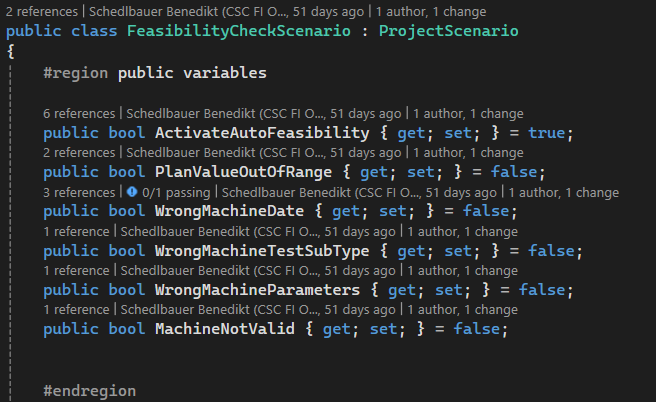
\includegraphics[width=1\textwidth]{bilder/unittests-parameters.png}
    \caption{Boolean-Parameter der \texttt{FeasibilityCheckScenario}-Klasse}
    \label{fig:unittests-parameters}
\end{figure}

Durch diese abstrahierte Vorgehensweise lassen sich die umfangreichen Unittests strukturiert und effizient umsetzen. Zwei Beispiel-Unittests sind in Abbildung~\ref{fig:unittestcases} dargestellt. Hierbei legt die Methode \texttt{CreateDefaultFeasibilityProject()} einen Default-Test an, der jeweils mit nur einer Operation und einem Parameter befüllt wird, um das Testszenario zu vereinfachen. Anschließend generiert die Methode \texttt{CreateMockData()} in der Datenbank alle erforderlichen ''Dummy-Daten'' bzw. passt bestehende Datensätze an, beispielsweise in der Feasibility-Konfigurationstabelle. Die Erstellung dieser ''Dummy-Daten'' erfolgt abhängig von den eingestellten \linebreak Boolean-Parametern, sodass die entsprechenden Szenarien erfüllt werden. Im zweiten Unittest, wie in Abbildung~\ref{fig:unittestcases} gezeigt, wurde beispielsweise das Szenario \texttt{WrongMachineDate} aktiviert. Danach wird über die Methode \texttt{PerformFeasibilityCheck()} der Feasibility Check ausgeführt, wobei das zurückgelieferte Ergebnis abschließend evaluiert wird. Ein automatisierter ''Cleanup-Mechanismus'' sorgt schließlich dafür, dass die initial angelegten ''Dummy-Daten'' sicher wieder aus der Datenbank entfernt werden.

\begin{figure}[!htb]
    \centering
    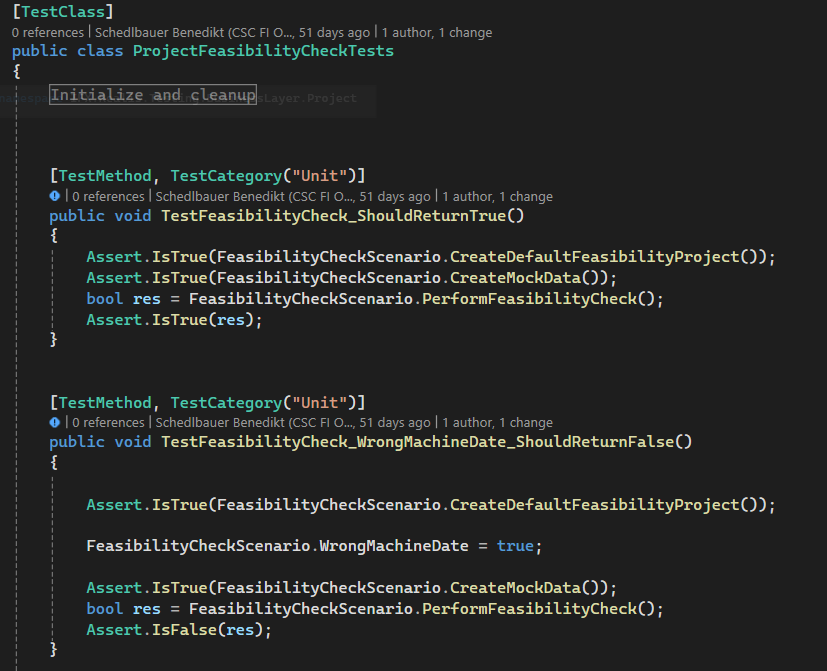
\includegraphics[width=1\textwidth]{bilder/unittestcases.png}
    \caption{Unittests für den Feasibility Check}
    \label{fig:unittestcases}
\end{figure}

Die Unittests sind in ein automatisiertes Test-Framework integriert, sodass bei jeder Änderung der Backend-Logik automatisch überprüft wird, ob alle Testfälle weiterhin erfolgreich durchlaufen werden. Diese Vorgehensweise unterstützt die kontinuierliche Qualitätssicherung und trägt maßgeblich zur Stabilität und Wartbarkeit des Systems bei.

\section{Ergebnisse der Tests}

Die umfangreichen Unittests haben wertvolle Einblicke in die Funktionsweise und Stabilität des Feasibility Checks geliefert. Die zentralen Erkenntnisse lassen sich wie folgt zusammenfassen:

\begin{itemize}
    \item \textbf{Standard-Szenario:} Bei korrekter Konfiguration und gültigen Eingabedaten wird der Feasibility Check ohne Fehlermeldungen abgeschlossen. Dies zeigt, dass die Standardlogik robust implementiert ist.
    \item \textbf{Spezifische Fehlerszenarien:} Durch die Aktivierung von Szenarien wie \texttt{PlanValueOutOfRange} und \texttt{WrongMachineDate} konnten gezielt Fehlerfälle simuliert werden. Die Tests bestätigten, dass diese Situationen korrekt erkannt und mit den vorgesehenen Fehlermeldungen quittiert werden.
    \item \textbf{Wiederholbarkeit:} Alle Testfälle lieferten bei wiederholter Durchführung konsistente Ergebnisse, was die Zuverlässigkeit der Testumgebung bestätigt.
\end{itemize}


\section{Evaluation des Systems}

Die Evaluation des Gesamtsystems stellt einen zentralen Bestandteil der Qualitätssicherung dar. Bislang lag der Fokus der Tests primär auf den Backend-Komponenten, wodurch indirekt auch die Datenbank validiert wurde. Die \texttt{FeasibilityCheckScenario}-Klasse bietet hierbei eine fundierte Basis für die zukünftige Implementierung spezifischer Anwendungsfalltests. Das Frontend wurde jedoch noch nicht in die Testprozesse einbezogen.

Um eine vollständige Validierung des Systems – bestehend aus Frontend, Backend und Datenbank – zu gewährleisten, ist die Entwicklung gezielter Unittests für das Frontend unerlässlich. Nur durch eine systematische Überprüfung aller Komponenten kann sichergestellt werden, dass diese fehlerfrei funktionieren und nahtlos miteinander interagieren.

Zusätzlich ist eine praxisorientierte Evaluation durch Endanwender von entscheidender Bedeutung. Durch Tests in realen Nutzungsszenarien können potenzielle Schwachstellen identifiziert und behoben werden. Ein iterativer Testprozess, der sowohl automatisierte als auch manuelle Tests integriert, gewährleistet, dass das System den Anforderungen des produktiven Einsatzes entspricht und kontinuierlich optimiert werden kann.
